\section{Tutorial de testing}
\label{sect:testing}

En este apartado se indican los pasos a seguir para poder ejecutar los tests de la aplicación sin complicaciones. Se recomienda hacer
la configuración necesaria en un sistema Unix ya que es donde se ha trabajado la aplicación y, más adelante, se indicará hacer uso de mandatos 
específicos de Unix.

\begin{enumerate}
	\item Lo primero es tener el proyecto actualizado. El repositorio debería ser accesible para cualquier usuario en 
            \href{https://github.com/Javiex7/Outsider}{github.com/Javiex7/Outsider}.
	\item Para la ejecución de los tests en indispensable la instalación tanto de Python \cite{installPython} como de Docker \cite{installDocker}.
	\item Con estos programas instalados en el sistema, es necesario acceder al repositorio para la configuración básica.
	\item Dentro del proyecto, son necesarios la instalación de varios elementos en el dispositivo, específicamente Django y los paquetes
	      pertinentes. Para evitar problemas, se recomienda descargar los elementos listados en el ``requirements.txt'' dentro de la carpeta principal
	      ``OutsiderProject''. Esta instalación se puede realizar fácilmente mediante el mandato: 
	      	                
	      pip install -r requirements.txt
	      	      
	\item A continuación, se requiere ejecutar un contenedor en Docker encargado de gestionar el servidor Redis para
	      que se haga uso en los tests. Mediante el siguiente mandato se puede poner en ejecución el servicio:
	      	      
	      docker run --rm -p 6379:6379 redis:7
	      	      
	\item Antes de poder ejecutar los tests, se debe configurar un variable de entorno para indicar el uso de 
	      este servidor Redis. Para ello habría que acceder a ``OutsiderProject/outsider/settings.py'' y modificar
	      el flag booleano denominado ``TEST'' y asegurarse que su valor sea True (línea 92).
	      	      
	\item Finalmente, el sistema puede ejecutar los tests. Para ello solo habría que ejecutar el mandato ``pytest''
	      desde el directorio padre, ``OutsiderProject''. Después de la ejecución debería mostrarse por consola
	      un resultado similar a lo que se puede visualizar en la Figura \ref{fig:res_testing}
	      	         
\end{enumerate}	

\begin{figure}[h]
	\centering
	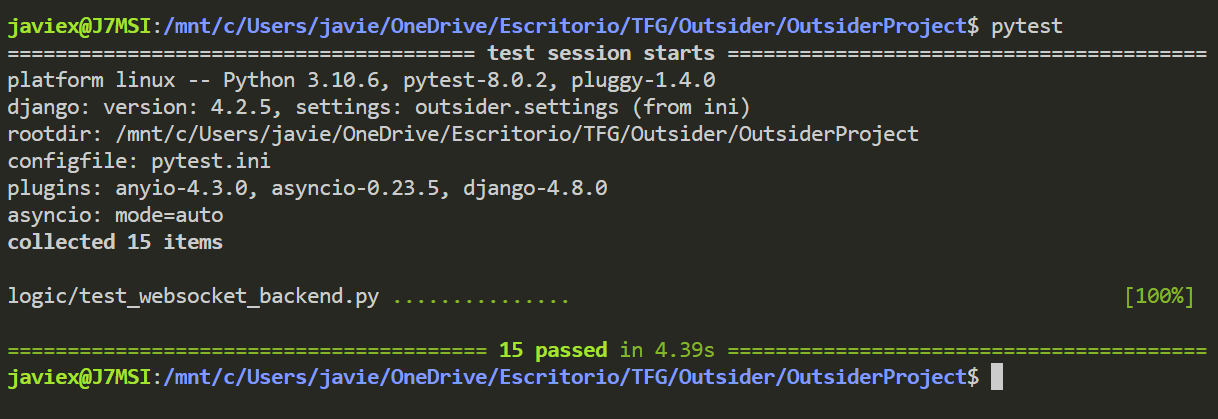
\includegraphics[width=\textwidth,clip=true]{res_testing.png}
	\caption{Ejecución de tests}
	\label{fig:res_testing}
\end{figure}

\section{Instrucciones de despliegue}
\label{sect:despliegue}

En este apartado se indican las instrucciones a la hora de realizar un despliegue de la aplicación a través de AWS. En el Código~\ref{alg:despliegue} se indican todos los mandatos que se deben ejecutar
y que se va a referenciar a continuación.

\begin{enumerate}
	\item En primer lugar, es necesario tener una máquina EC2 preparada para poder conectarse a ella. En la Figura \ref{fig:res_despliegue} se puede
		  observar el panel de control de EC2 de AWS. Desde este panel se pueden lanzar nuevas instancias y gestionar las que ya han sido configuradas
		  y lanzadas anteriormente. Para este proyecto se está haciendo uso de la máquina nombrada como ``outsider-machine''
	\item Con la máquina lista, es necesario conectarse a ella mediante el uso del mandato ssh y las claves privadas generadas
		  a la hora de crear la instancia de la máquina.
		  Se destaca que se debe sustituir ``machineDir'' por la dirección DNS de la máquina en cuestión. Esta dirección y demás información
		  relacionada con la conexión a una máquina EC2 se puede encontrar en la sección de ``Conectarse a una instancia'' dentro de la página de 
		  gestión de EC2.
	\item Ya en el directorio principal, se puede crear una carpeta adicional o descargar el repositorio del código directamente. 
	      El repositorio debería ser accesible para cualquier usuario en \href{https://github.com/Javiex7/Outsider}{github.com/Javiex7/Outsider} y para descargarlo desde 
		  la terminal simplemente es necesario hacer uso del mandato ``git clone''.
	\item Ahora solo quedaría acceder al directorio principal y ejecutar el mandato de Docker para ejecutar los contenedores
		  descritos en el fichero ``docker-compose.yaml''.
	\item Después del tiempo de descarga e instalación necesario, la aplicación estará lista para su uso mientras se mantenga activa la
		  máquina EC2.
\end{enumerate}	

\begin{mypython}[float={h},caption={Mandatos de consola para el despliegue},label={alg:despliegue}]
	sudo ssh -i "privatekeys.pem" ubuntu@machineDir...

	git clone https://github.com/Javiex7/Outsider.git
	
	cd Outsider/OutsiderProject
	sudo docker compose -f docker-compose.yaml up --build
\end{mypython}

\begin{figure}[h]
	\centering
	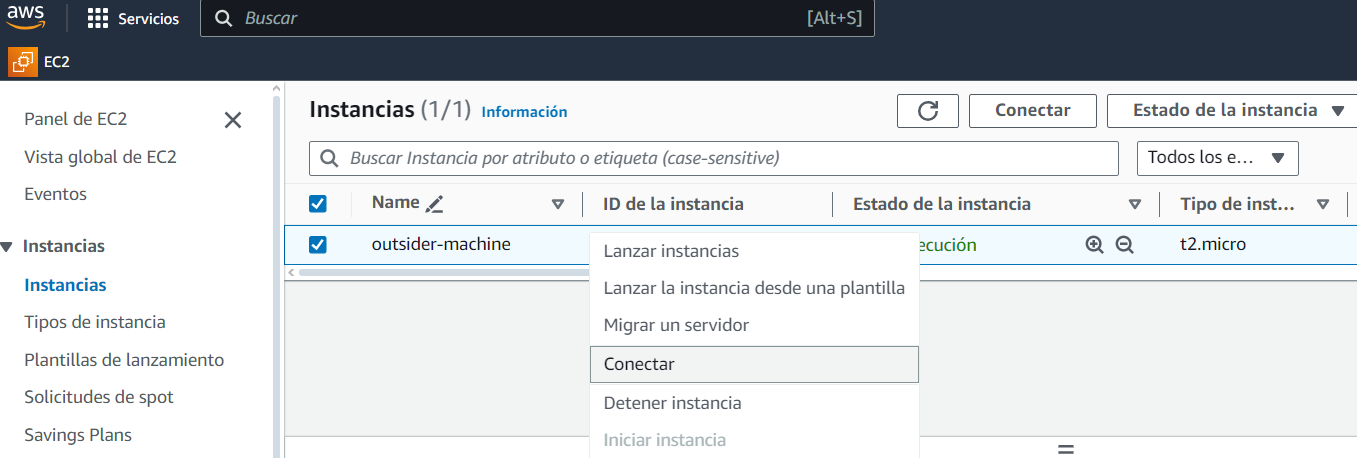
\includegraphics[width=\textwidth,clip=true]{res_despliegueAWS.png}
	\caption{Panel de control de EC2}
	\label{fig:res_despliegue}
\end{figure}